\section{Background and Motivation}
\label{back}
%In this section, we discuss the Docker containers' framework and SwarmKit, the default cluster management tool.
\subsection{Docker Containers}
%Container technology or containerization is an virtualization method for 
%deploying and running distributed applications without launching an entire virtual machine for each of them.  
%Instead, multiple isolated service units of the application, called containers, are sharing the host operating system and physical resources.
%The concept of container virtualization is yesterday's news; Unix-like operating systems leveraged the technology for over a decade. 
%However, new containerization platforms, such as Docker, make it into the mainstream of application development.
%Based on previously available open-source technologies (e.g. cgroup), Docker introduces a way of simplifying the tooling required to create and manage containers.

A Docker worker machine runs a local Docker daemon. 
New containers may be created on a worker by sending commands to its local daemon, such as \replaced{\texttt{docker run -it ubuntu bash}}{``docker
	run -it ubuntu bash''}. \added{Not sure how IEEE format wants in-line code examples. Further, what journal are we aiming for, and how do they want things? I should look at their templates.}
A Docker container image is a lightweight, stand-alone, executable package of a piece of software that 
includes everything needed to run it: code, run-time, system tools, system libraries, and settings.
In general, each container targets a specific service of an application. If the application needs to scale up this particular service, 
it initiates duplicated containers by using the same image. One physical machine can host many applications with various services in a standalone mode.

\begin{comment}
\begin{figure}[ht]
\centering
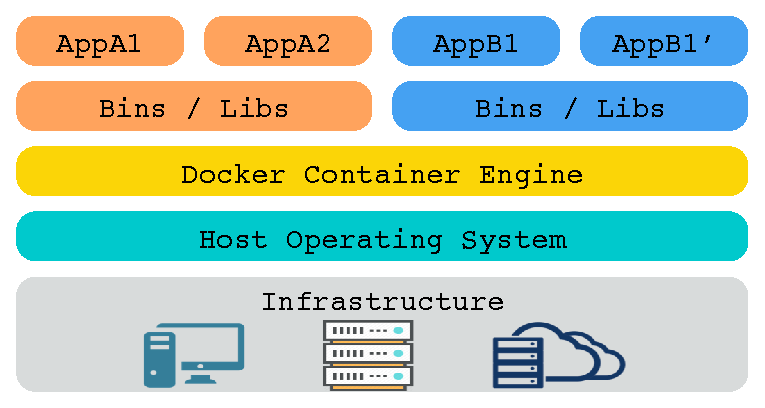
\includegraphics[width=0.75\linewidth]{docker-standalone}
\caption{Docker Containers}
\label{fig:docker-standalone} 
\end{figure}
\end{comment}

\begin{comment}
Fig~\ref{fig:docker-standalone} illustrates the structure of a physical machine 
that is hosting four Docker containers for two applications. As the figure shows, the $AppA$ includes two services that are provided by $AppA1$ and $AppA2$ 
and $AppB$ contains one service which is provided by two Docker containers, $AppB1$ and $AppB1\textprime$.


%\begin{comment}
\begin{figure}[ht]
%\hspace*{0.8in}
   \centering
%\vspace{-0.1in}
      \begin{minipage}[t]{0.48\linewidth}
\centering
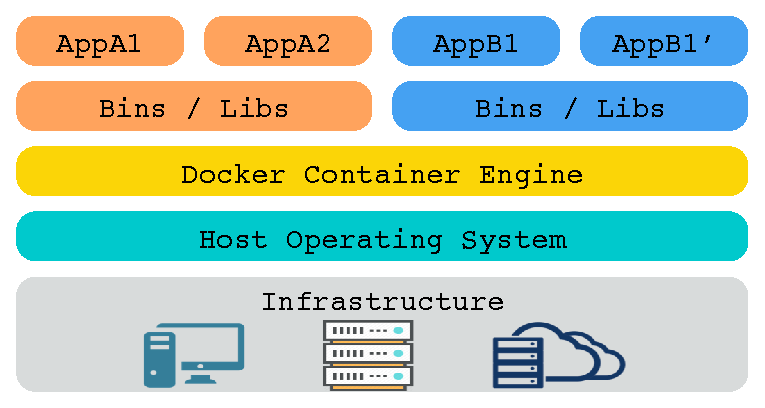
\includegraphics[width=\linewidth]{docker-standalone}
\caption{Docker Containers}
\label{fig:docker-standalone}
      \end{minipage} %
      %%%%%%%%%%%%%%%%%%%%%%%%%%%%%%%%
      \begin{minipage}[t]{0.48\linewidth}
\centering
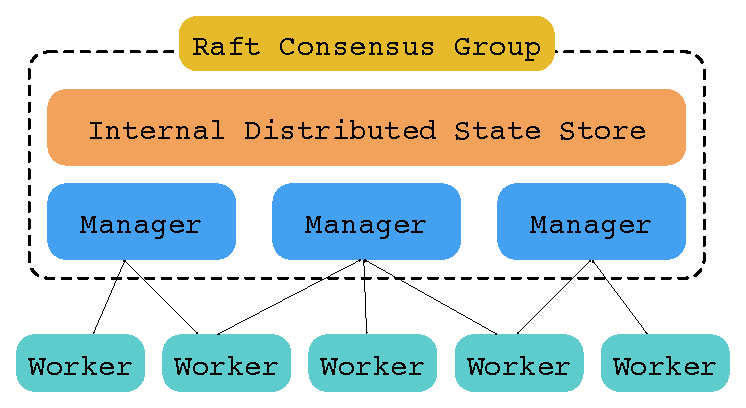
\includegraphics[width=\linewidth]{swarmkit}
\caption{Docker Swarmkit}
\label{fig:swarmkit} 
      \end{minipage} %
%\caption{Resource demonds under different workloads on four services, MySQL, Tomcat, YUM, PI.}
\end{figure}
%\end{comment}


\begin{comment}
\begin{figure}[ht]
\centering
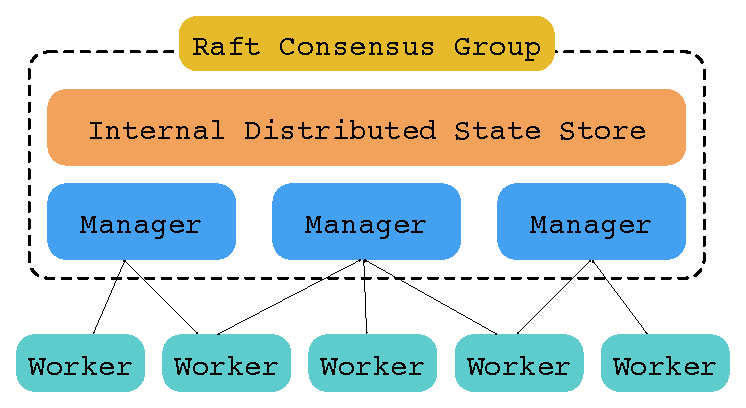
\includegraphics[width=0.8\linewidth]{swarmkit}
\caption{Docker Swarmkit}
\label{fig:swarmkit} 
\end{figure}
\end{comment}


\subsection{Container Orchestration}
When deploying applications into a production environment, it's difficult to achieve resilience and scalability on a single container host. 
Typically, a multi-node cluster is used to provide the infrastructures for running containers at scale. Introduced by Docker, SwarmKit is an open source toolkit
for container orchestration in the cluster environment. 

There are two types of nodes in a cluster that are running SwarmKit, worker nodes, and manager nodes.
Worker nodes are responsible for running tasks; on the other hand, 
manager nodes accept specifications from the user and are responsible for reconciling the desired state with the actual cluster state. \added{[we need to say abit more about what that means. What about the state could be 
	undesired vs desired?]}
%Fig.~\ref{fig:swarmkit} shows the decentralized architecture of a SwarmKit cluster. 
%A manager node is in charge of several worker nodes and there is a overlap between 
%manager nodes to tolerate failures. Worker and manager nodes are equal in the system since a worker node can be promoted to a manager and a manager node 
%can be demoted to a worker. Manager nodes are formed into a Raft consensus group to maintain global cluster's states. 
%The Raft consensus algorithm is used to ensure that all the manager nodes that are in charge of managing and 
%scheduling tasks in the cluster are storing the same consistent states. 

\added{[What is the point of this paragraph? We just jump in saying we can set limits at init time. (Note that we can also update them with \texttt{docker update ...}). Is this even relevant for this paper, since we are 
	talking about container \textit{placement} which is a cluster-level, rather than container-level, decision process]} A Docker container can be initiated with specific requirements (e.g. memory and CPU) and user-defined labels.
The scheduler that runs on a manager combines the user-input information with states of each node to make various scheduling decisions, 
such as choosing the best node to perform a task. \added{[We may need a more clear example of what a 'task' is]}
Specifically, it utilizes filters and scheduling strategies to assign tasks. \added{[What is a filter? Would someone in this field know that or do we need to define? I certainly don't know.]}
There are four filters available.
\emph{ReadyFilter:} checks that the node is ready to schedule tasks;
\emph{ResourceFilter:} checks that the node has enough resources available to run;
\emph{PluginFilter:} checks that the node has a specific volume plugin installed.
\emph{ConstraintFilter:} selects only nodes that match certain labels.
If there are multiple nodes that pass the filtering process, 
SwarmKit supports three scheduling strategies: spread (currently available), binpack, and random (under development based on Swarm Mode). \added{[Is this still the case? I know its been a while since this project was last touched.]}
\emph{Spread strategy:} places a container on the node with the fewest running containers.
\emph{Binpack strategy:} places a container onto the most packed node in the cluster.
\emph{Random strategy:} randomly places the container into the cluster.

\begin{figure}[ht]
\centering
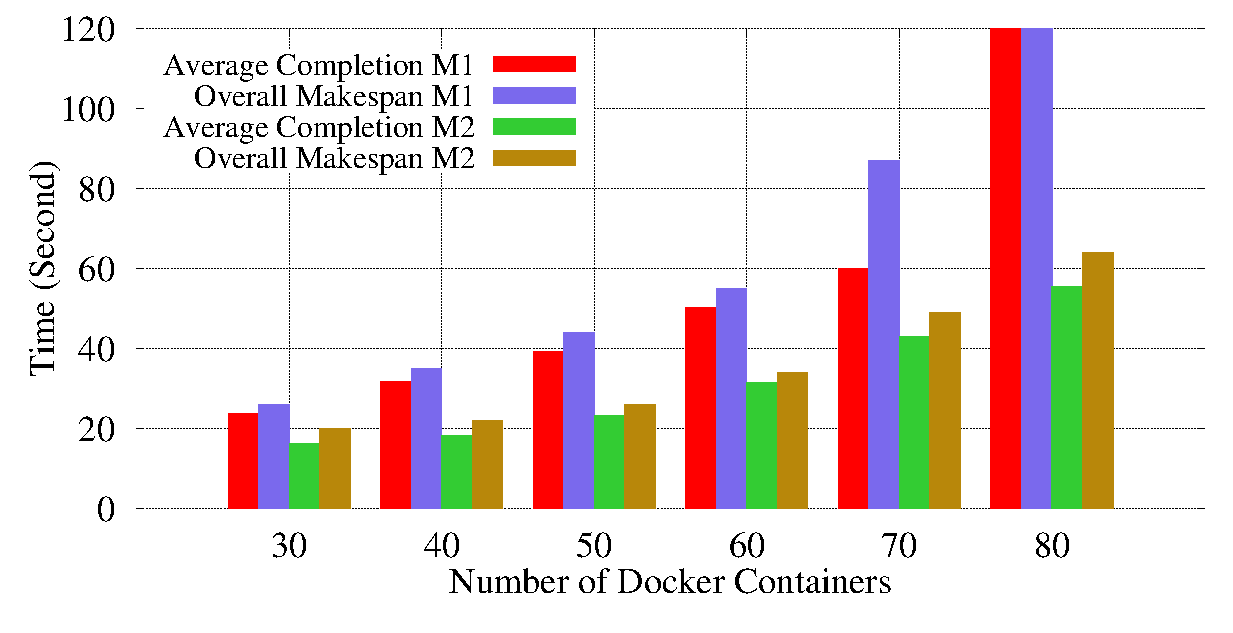
\includegraphics[width=0.8\linewidth]{start-single}
\caption{Starting Dockers on a single machine}
\label{fig:start-single} 
\end{figure}

The default spread strategy, which 
attempts to schedule a service task based on the number of active containers on each node, 
can roughly assess the resources on the nodes. 
However this assessment fails to reflect various nodes in a heterogeneous cluster setting.
Considering the heterogeneity, the nodes in such a cluster have different configurations in terms of memory, CPU, and network.
Therefore, running the same amount of containers on these nodes results in different experiences.
Fig~\ref{fig:start-single} plots the average starting delay of and overall makespan of the set of Tomcat Docker containers. 
We conduct the experiments on two machines, M1 with 8GB memory, 4-core CPU and M2 has
16GB memory and 8-core CPU. On each particular machine, M1 or M2, we can see that the more containers it hosts, the larger the starting delay 
and makespan. However, M1 costs 23.67s on average to start 30 Tomcat containers and M2 costs 18.32s to start 40 containers. 
Additionally, when trying to initiate 80 Tomcat containers, M1 fails to complete the job and M2 finishes it. \added{[So, is the point here that the nodes arent 'heterogenous' and that \#containers may not be a good way to decide which node is ready to handle a new task? That seems reasonable to me. We should say so explicitly]}




